\documentclass[tikz,border=8pt]{standalone}
\usepackage{amsmath}
\usetikzlibrary{arrows.meta}
\definecolor{ink}{HTML}{21352F}
\definecolor{teal}{HTML}{087F7B}
\definecolor{blue}{HTML}{4B77A8}
\definecolor{gold}{HTML}{C58B2A}
\definecolor{rose}{HTML}{B65A62}
\begin{document}
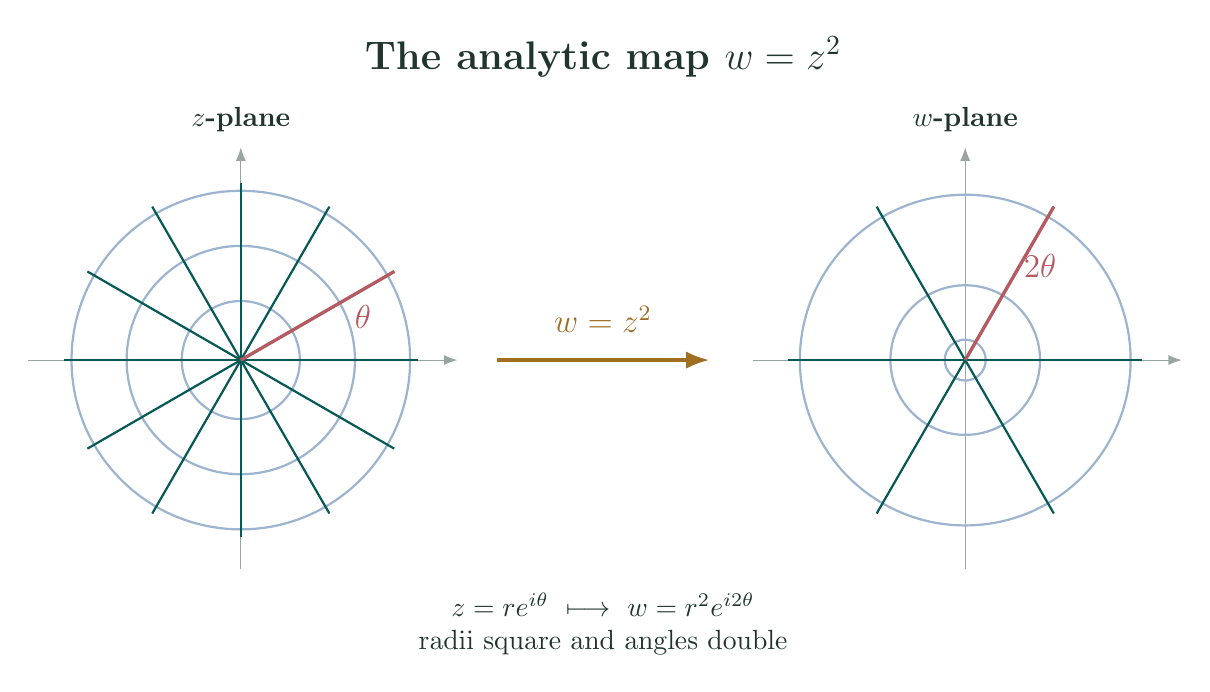
\begin{tikzpicture}[font=\large\sffamily,text=ink,>=Latex]
  \node[font=\bfseries\Large] at (0,3.85)
    {The analytic map $w=z^2$};

  \begin{scope}[xshift=-4.6cm]
    \node[font=\bfseries] at (0,3.05) {$z$-plane};
    \draw[->,ink!45] (-2.7,0)--(2.75,0);
    \draw[->,ink!45] (0,-2.65)--(0,2.7);
    \foreach \r in {.75,1.45,2.15}
      \draw[blue!55,thick] (0,0) circle (\r);
    \foreach \a in {0,30,...,150}
      \draw[teal!70!black,thick] ({-2.25*cos(\a)},{-2.25*sin(\a)})
        --({2.25*cos(\a)},{2.25*sin(\a)});
    \draw[rose,very thick] (0,0)--({2.25*cos(30)},{2.25*sin(30)});
    \node[rose] at (1.55,.55) {$\theta$};
  \end{scope}

  \draw[gold!80!black,very thick,->] (-1.35,0)--(1.35,0)
    node[midway,above=6pt] {$w=z^2$};

  \begin{scope}[xshift=4.6cm]
    \node[font=\bfseries] at (0,3.05) {$w$-plane};
    \draw[->,ink!45] (-2.7,0)--(2.75,0);
    \draw[->,ink!45] (0,-2.65)--(0,2.7);
    \foreach \r in {.26,.95,2.1}
      \draw[blue!55,thick] (0,0) circle (\r);
    \foreach \a in {0,60,120}
      \draw[teal!70!black,thick] ({-2.25*cos(\a)},{-2.25*sin(\a)})
        --({2.25*cos(\a)},{2.25*sin(\a)});
    \draw[rose,very thick] (0,0)--({2.25*cos(60)},{2.25*sin(60)});
    \node[rose] at (.95,1.2) {$2\theta$};
  \end{scope}

  \node[font=\normalsize,align=center] at (0,-3.35)
    {$z=re^{i\theta}\ \longmapsto\
      w=r^2e^{i2\theta}$\\
     radii square and angles double};
\end{tikzpicture}
\end{document}
